\documentclass{article}
\usepackage{amsmath}
\usepackage{graphicx}
\usepackage{booktabs}
\title{ECE 565 Project}
\author{Luc Bouchard}

\begin{document}
\maketitle


\begin{equation}    
\begin{aligned}
    &(\vec{x}_i, y_i) \quad i \in 1,2,3...n \\
    &X \in ~ N(0, \sigma^2I_d) \\
    &Y \in ~ {0, 1}
\end{aligned}
\end{equation}

\section{Model}

\begin{equation}
    P(y = 1|\vec{x}; \vec{w}) = \frac{e^{\vec{w}^T\vec{x}}}{1 + e^{\vec{w}^T\vec{x}}}
\end{equation}

\section{Parameters}

\begin{equation}    
    \begin{aligned}
        &\vec{\theta} = \vec{w} \\
        &\vec{y} = [y_1, y_2, y_3, .... y_n]^T
    \end{aligned}
\end{equation}

\section{Liklihood Function}

\begin{equation}
    f(y_1 ... y_n; \vec{w}) = \prod_{i = 1}^{n} \Big(\frac{e^{\vec{w}^T\vec{x}_i}}{1 + e^{\vec{w}^T\vec{x}_i}}\Big)^{y_i} \Big(1 - \frac{e^{\vec{w}^T\vec{x}_i}}{1 + e^{\vec{w}^T\vec{x}_i}}\Big)^{1 - y_i}
\end{equation}

\section{CRLB}

\begin{equation}
    CRLB = I(\theta)^{-1}
\end{equation}

\begin{equation}
    I_{ij}(\vec{w}) = -E_Y\Big[\frac{\partial^2\log{f(y_1...y_n; \vec{w})}}{\partial w_i \partial w_j}\Big]
\end{equation}

Note

\begin{equation}
    \frac{\partial^2\log{f(y_1...y_n; \vec{w})}}{\partial w_i \partial w_j} = \sum_{z = 1}^{n}\frac{\partial \log f(y_z|\vec{x}_z;\vec{w})}{\partial w_i \partial w_j}
\end{equation}

Consider $f(y|\vec{x};\vec{w})$,

\begin{equation}
    f(y|\vec{x}; \vec{w}) = \Big(\frac{e^{\vec{w}^T\vec{x}}}{1 + e^{\vec{w}^T\vec{x}}}\Big)^{y} \Big(1 - \frac{e^{\vec{w}^T\vec{x}}}{1 + e^{\vec{w}^T\vec{x}}}\Big)^{1 - y}
\end{equation}

\begin{equation}
    f(y|\vec{x}; \vec{w}) = \Big(\frac{e^{\vec{w}^T\vec{x}}}{1 + e^{\vec{w}^T\vec{x}}}\Big)^{y} \Big(\frac{1}{1 + e^{\vec{w}^T\vec{x}}}\Big)^{1 - y}
\end{equation}

\begin{equation}
    \log f = y\vec{w}^T\vec{x} - \log(1 + e^{\vec{w}^T\vec{x}})
\end{equation}

\begin{equation}
    \frac{\partial \log f}{\partial w_i} = x_i \Big( y - \frac{e^{\vec{w}^T\vec{x}}}{1 + e^{\vec{w}^T\vec{x}}} \Big)
\end{equation}

\begin{equation}
    \frac{\partial^2 \log f}{\partial w_i\partial w_j} = -P(y = 1|\vec{x}; \vec{w})\ P(y = 0|\vec{x}; \vec{w})\ x_ix_j
\end{equation}

Note that equation (12) has no $y$ dependence, so the expectation is trivially computed:

\begin{equation}
    E_Y\Big[\frac{\partial^2 \log f}{\partial w_i\partial w_j}\Big] = -P(y = 1|\vec{x}; \vec{w})\ P(y = 0|\vec{x}; \vec{w})\ x_ix_j
\end{equation}

\begin{equation}
    E_Y\Big[\frac{\partial^2 \log f}{\partial \vec{w}^2}\Big] = -P(y = 1|\vec{x}; \vec{w})\ P(y = 0|\vec{x}; \vec{w})\ \vec{x}\vec{x}^T
\end{equation}

Finally,

\begin{equation}
    I(\vec{w}) = \sum_{i = 0}^n P(y = 1|\vec{x}_i; \vec{w})\ P(y = 0|\vec{x}_i; \vec{w})\ \vec{x_i}\vec{x_i}^T
\end{equation}

\section{Consider 1D Case ($d = 1$, $x \in R, w \in R$)}

\begin{equation}
    var(\hat{w}) \geq \Big( \sum_{i=1}^{n} x_i^2\ P(y = 1|x_i; w)\ P(y = 0|x_i; w) \Big)^{-1}
\end{equation}

Note that $w$ in the equation above is the true $w$, and $\hat{w}$ is the estimate for $w$.

Let's assume all $x_i = 1$. This reduces equation (16) to the following:

\begin{equation}
    var(\hat{w}) \geq \frac{1}{n \Big(\frac{e^w}{1+e^w}\Big)\Big(\frac{1}{1+e^w}\Big)} = \frac{(1 + e^w)^2}{ne^w}
\end{equation}

\begin{figure}[h!]
    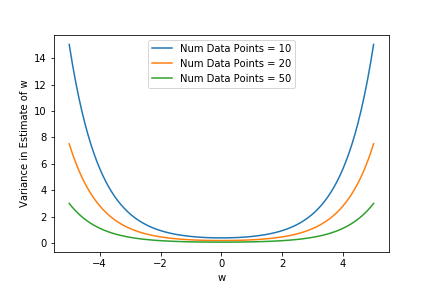
\includegraphics[width=\linewidth]{out.png}
\end{figure}

\end{document}